\section{Introduction}
Metro maps, circuits, networks, construction plans and many more - they all can be visualized with a corresponding \textit{graph drawing}. Over the last decades, many different efficient algorithms were developed for graph drawings in the Euclidean plane. Especially, orthogonal graph drawings are of interest as they are applicable in various fields.
\\In order to work with graph drawings efficiently, one has to consider the \textit{quality} of a graph drawing. There is a huge variety of aspects to consider when we want to examine the quality of a drawing. The readability of the illustrated information, the size of the drawing - measured with the pair of vertices with the farthest distance in the drawing, and the \textit{edge complexity} - the amount of consecutive line segments for an edge illustration are only a few aspects how to measure the drawing quality. Naturally, we try to create drawings as clearly as possible meaning to avoid drawings with a high edge complexity. If a given graph admits a \textit{crossing-free}, or in other words \textit{planar} drawing, we want to preserve this property in further processing approaches.
\\The American abstract artist \textit{Mark Lombardi} gained approval for his aesthetic illustration of political-economic structures. The diagrams included \textit{circular arcs} of different sizes and their even distribution around a vertex in order to vizualize connections adequately. It seems that the circular arcs emphasize the connection between components in sense of direction.
\begin{figure}[H]
	\centering
	\begin{subfigure}{\textwidth}
		\centering
		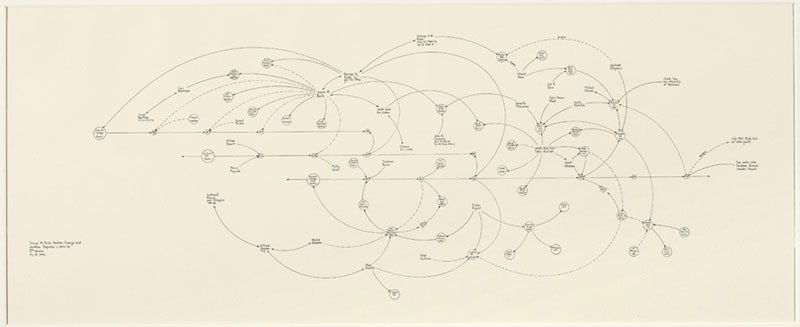
\includegraphics[width=0.8\linewidth]{includegraphics/Introduction_Lombardi-example}
	\end{subfigure}
\caption{Work of Mark Lombardi \cite{lombardi_ex}}\label{im:lombardi_ex}
\end{figure}
\textit{Orthogonal drawings} arise among others in VLSI design where quite many cables are following a similar path. The smallest angle between axis-aligned line segment is at most $\pi/2$ and their angular resolution is quite pleasing for the eye of the viewer. One fundamental, reliable model is the \textit{Kandinsky model} which is based on a \textit{grid embedding}. The vertices lie on a \textit{coarse} grid while the edges lie on a \textit{fine} grid extending the coarse grid. It may appear that an orthogonal drawing may convey some structural information, so \textit{smoothening} those edges is of interest. In this thesis, we focus on the smoothening of Kandinsky drawings by introducing circular arcs, inspired by \textit{Lombardi drawings} as illustrated in Figure \ref{im:lombardi_ex}\cite{lombardi_src1}\cite{lombardi_src2}. 
\begin{figure}[H]
	\centering
	\begin{subfigure}{0.45\textwidth}
		\centering
		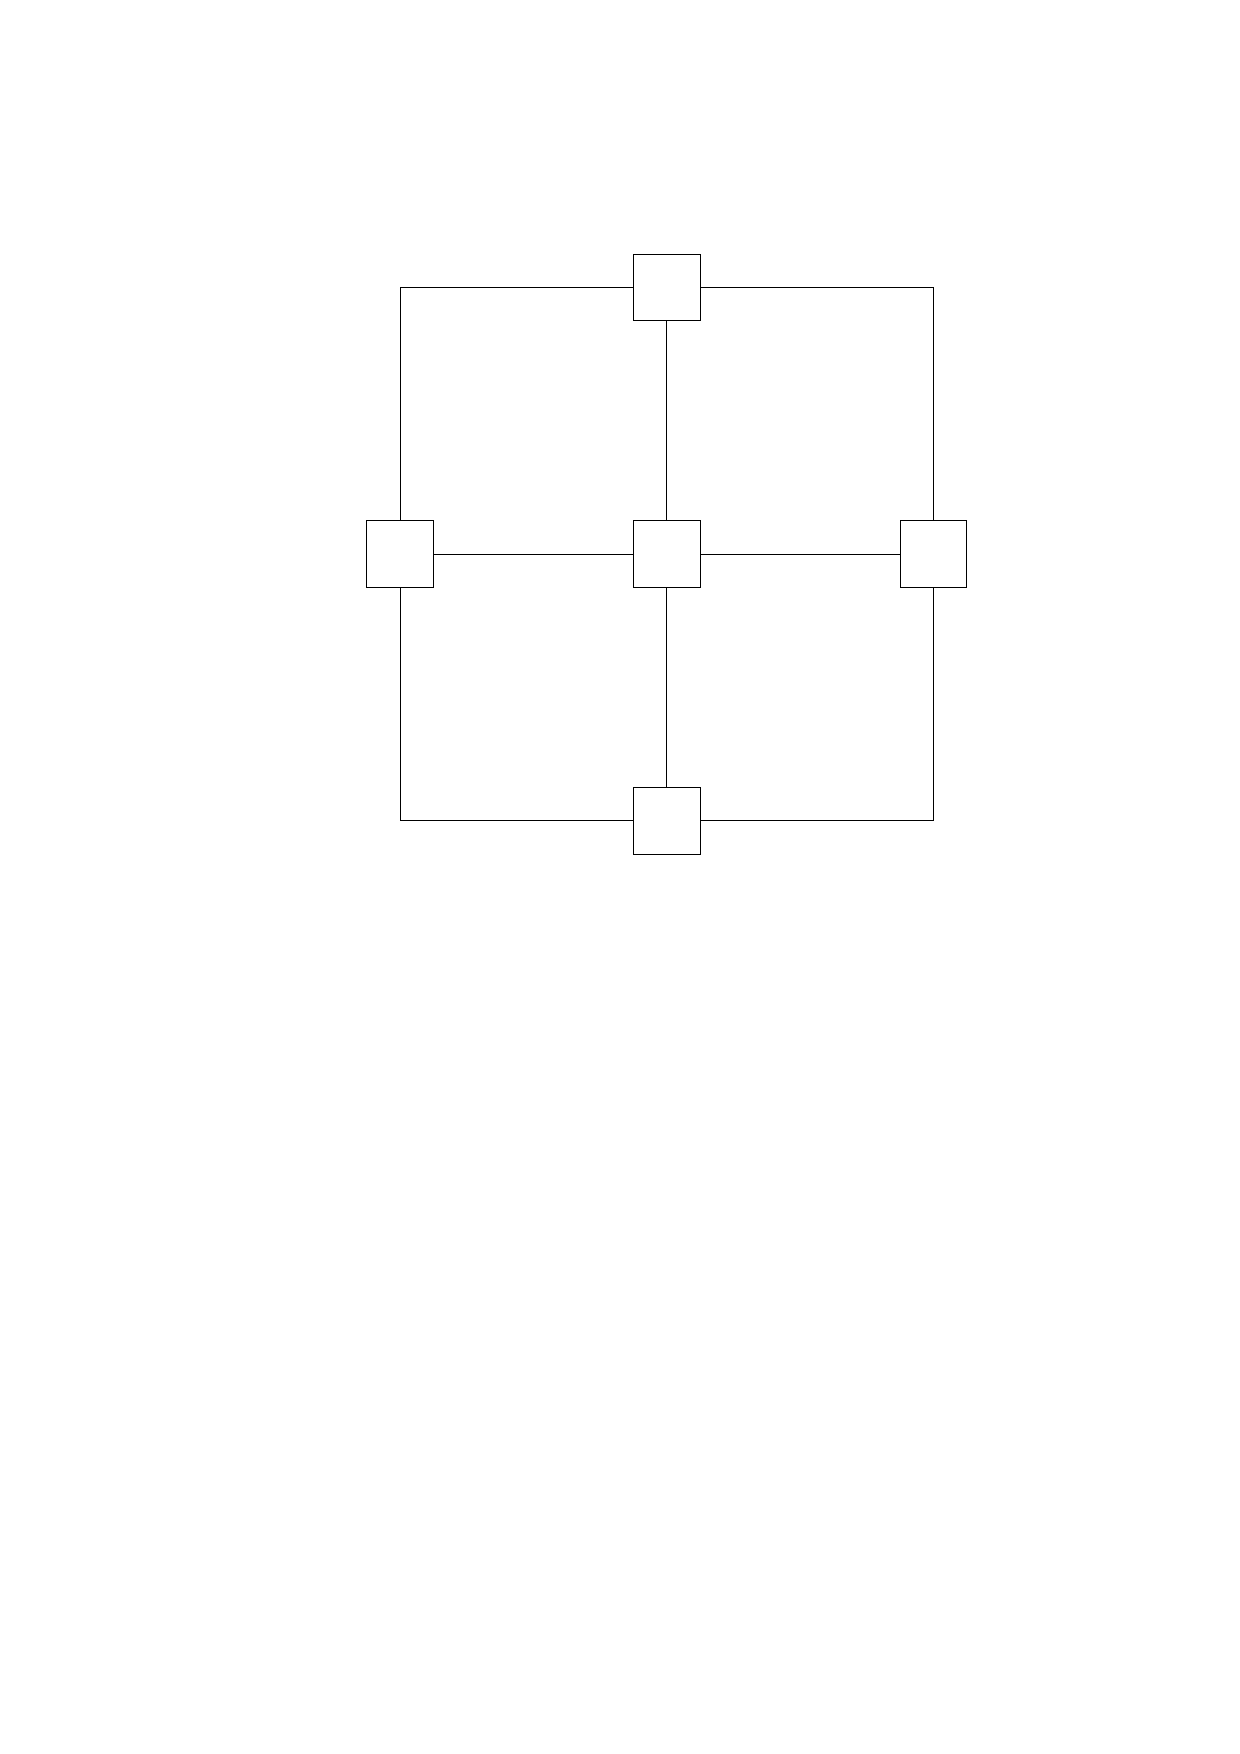
\includegraphics[width=0.4\linewidth,page=1]{includegraphics/introduction-example}
		\caption{Orthogonal drawing}\label{im:introduction_ex1}
	\end{subfigure}
	\begin{subfigure}{0.45\textwidth}
		\centering
		\includegraphics[width=0.4\linewidth,page=2]{includegraphics/introduction-example}
		\caption{Smoothened drawing}\label{im:introduction_ex2}
	\end{subfigure}
	\caption{Smoothening a drawing for aesthetic appeal}
\end{figure}
By postprocessing an input drawing like illustrated in Figure \ref{im:introduction_ex1} and \ref{im:introduction_ex2}, we also have to consider possible shape alternations. It is desirable that the orientation of the vertices is preserved, meaning that e.g. a metro map can still be read reasonably after the smoothening process\cite{metro1}.\\
However, it is a priori not guaranteed that there is a smoothening for every input Kandinsky drawing with a reasonable complexity increase. The introduction of circular arcs might arise some conflicts in sense of planarity. Dealing with postprocessing algorithms, we have to focus on new area bounds and the behaviour of the edge complexity in order to quantify the resulting quality of the smoothened drawing.